%!TEX root=main.tex
\section{Background}
\label{kvdirect:sec:background}


\egg{
\subsection{The Road to High Performance Key-Value Storage}

Building a high performance key-value storage is a non-trivial exercise of optimizing various software and hardware components in a computer system. The rich literature on key-value storage performance optimizations can give us a glimpse of software and hardware evolution in recent years.
Early works on distributed in-memory key-value storage such as Memcached~\cite{fitzpatrick2004distributed} uses OS locks for multi-core synchronization and TCP/IP networking stack for communication. Since then, optimizations have been made on multiple fronts to remove bottlenecks in various parts of the system.


\subsubsection{Synchronization cost}
\label{kvdirect:sec:CoreSynchronizationCost}
Synchronization is needed in multi-threaded key-value storage implementation since multiple clients might access the same keys concurrently. For example, when two clients make atomic increments to a single key, the value needs to reflect both increments.

To reduce synchronization cost, Masstree~\cite{mao2012cache}, MemC3~\cite{fan2013memc3} and libcuckoo~\cite{li2014algorithmic} optimize caching, hashing and memory allocation algorithms, and replace permissive kernel locks with optimistic version-based locks.
MICA~\cite{lim2014mica, li2016full} takes a further step to completely avoid synchronization by partitioning the hash table to each core so that each core serves an exclusive portion of the hash table.
This approach, however, may introduce core imbalance for long-tail access patterns with a few extremely popular keys~\cite{li2016full}.

\subsubsection{Networking overhead}
\label{kvdirect:sec:ReduceNetworkingOverhead}

In a key-value storage where computation to communication ratio is low, a significant portion of CPU cycles is spent in the kernel networking stack, including protocol handling, memory copy, system call and multi-core synchronization~\cite{peter2016arrakis}.
Furthermore, the kernel network stack adds hundreds of microseconds latency~\cite{ousterhout2015ramcloud}, which greatly impacts response time.
and complicates latency-hiding programming of applications that require multiple round-trips to the key-value storage.

Extensive research has been conducted to reduce network communication costs and improve end-to-end latency. One line of work proposes that key-value storage server software communicates directly with network cards by polling while bypassing the kernel~\cite{rizzo2012netmap, intel2014data}; packets are processed by a lightweight network stack in user space~\cite{jeong2014mtcp, marinos2014network}. Chronos~\cite{kapoor2012chronos}, RAMCloud~\cite{ousterhout2010case, ousterhout2015ramcloud} and MICA~\cite{lim2014mica,li2016full} leverage this approach to achieve high throughput (approximately 5 million key-value operations per second (op/s) per core) and low latency (microsecond-scale) by reducing networking overhead.

The other line of work leverages two-sided RDMA~\cite{infiniband2000infiniband} as an RPC mechanism between key-value storage client and server. RDMA is a hardware-based transport that almost completely removes the CPU overhead of networking. Key-value storage systems such as HERD~\cite{kalia2014using, kalia2016design} achieve per-core throughput and end-to-end latency comparable or superior to the first line of work, but the overall throughput per server largely depends on the processing capacity of RDMA network cards~\cite{kalia2016design}.

\subsubsection{Throughput bottleneck of CPU}
\label{kvdirect:sec:CPU-键值-Bottleneck}
When pushed to the limit, in high performance key-value storage systems the throughput bottleneck can be attributed to the computation in key-value operation and the latency in random memory access. Key-value storage needs to spend CPU cycles for key comparison and hash slot computation. Moreover, key-value storage hash table is orders of magnitude larger than the CPU cache, therefore the memory access latency is dominated by cache miss latency for practical access patterns.

By our measurement, a 64-byte random read latency for a contemporary computer (Sec.~\ref{kvdirect:sec:evaluation-setup}) is approximately 110~ns. A CPU core can issue several memory access instructions concurrently when they fall in the instruction window, limited by the number of load-store units in a core (measured to be 3 to 4 in our CPU)~\cite{gharachorloo1992hiding, han2010packetshader, zhang2015mega}. In our CPU, we measure a max throughput of 29.3M random 64B access per second per core. On the other hand, an operation to access 64-byte key-value pair typically requires approximately 100ns computation or approximately 500 instructions, which is too large to fit in the instruction window (measured to be 100 to 200). When interleaved with computation, the performance a CPU core degrades to only 5.5 MOps. An optimization is to batch memory accesses in a key-value store by clustering the computation for several operations together before issuing the memory access all at once~\cite{li2016full, narula2014phase}. This improves the per-core throughput to 7.9 MOps in our CPU, which is still far less than the throughput of the host DRAM. 


\begin{comment}
When pushed to the limit, in high performance key-value storage systems the throughput bottleneck can be attributed to the computation in key-value operation and the latency in random memory access. This is actually the bottleneck we want to remove in our design and we discuss the issue here in more detail. 

Key-value storage needs to spend CPU cycles for key comparison and hash slot computation. Moreover, key-value storage hash table is orders of magnitude larger than the CPU cache, therefore the memory access latency is dominated by cache miss latency for practical access patterns.

The latency for CPU to access DRAM on the same NUMA node, \ie cache miss latency, is 80\approx90 nanoseconds on our platform (measured with~\cite{intelmemaccess}, hardware details in sec. \ref{kvdirect:sec:implementation}).
For 64-byte access granularity, the random read latency including data copy is \approx110~ns.
This latency can be partially hidden by the out-of-order execution engine in modern CPUs, which can issue a few memory accesses in parallel.
However, the parallelism is limited by two factors: the number of load-store units (LSUs) per core~\emph{k} (measured to be 3\approx4 on our CPU) and the instruction window size~\emph{W} (measured to be 100\approx200 instructions on our CPU)~\cite{gharachorloo1992hiding, han2010packetshader, zhang2015mega}. When there are enough memory operations in the instruction window, \emph{k} of them can be issued simultaneously. 

Figure~\ref{kvdirect:fig:cpu-mem} shows random memory access performances of a multicore CPU. It shows that a modern CPU core can provide fairly high random memory access throughput (27M~op/s or 1.7~GB/s for 64B granularity). Moreover, memory throughput scales linearly with number of CPU cores, indicating that the DDR main memory is not a bottleneck.

However, in a key-value store memory access is interleaved with computation for hash slot calculation and key comparison. An operation to access a 64-byte key-value pair typically requires \approx100 ns computation or \approx500 instructions, which is far larger than the instruction window size.
Consequently, when the random memory access instructions for different keys are separated by computation, the second DRAM access is too far to fit in the same instruction window with the first DRAM access and cannot be issued in parallel.
\end{comment}

One can batch memory accesses in a key-value store, i.e., clustering the computation for several operations together before issuing the memory access all at once~\cite{li2016full, narula2014phase}.
Table~\ref{kvdirect:tab:kv-cpu-throughput} depicts the measured per-core hash table throughput under different key-value sizes and batch sizes, assuming the key-value is inlined in hash table and each key-value operation requires one non-cached memory access.
The results fit the following formulas within 10\% error:
\begin{equation}
%\small
\frac{1}{RandAccessThroughput} = \frac{MemLatency}{Parallelism}
\end{equation}
\begin{equation}
%\small \frac{1}{键值Throughput} = ComputeTime + \frac{MemLatency}{min(BatchSz, Parallelism)}
\begin{aligned}
\frac{1}{KeyValueOpThroughput} = & ComputationTime + \\
      & \frac{MemLatency}{min(BatchSize, Parallelism)}
\end{aligned}
\end{equation}
This indicates that when interleaved with computation, the performance of CPU degrades significantly. In the extreme case, even if the instruction window size or memory fetch parallelism goes to infinity, the per-core key-value operation throughput would still be bounded by computation (\approx10M~op/s), 10\approx20x slower than a single DDR channel.
\end{comment}

\egg{
\subsection{Domain-Specific Architectures for Key-Value Storage}

Ten years ago, processor frequency scaling was over and people turned to multi-core and concurrency~\cite{sutter2005free}.
Nowadays, CMOS feature-size reduction is getting more and more difficult, which implies that multi-core scaling is also over. People are turning to domain-specific architectures (DSAs)~\cite{esmaeilzadeh2013power} for better performance. Several such DSAs have been used to improve key-value storage performances. 

\egg{
For computation, DSAs such as GPU, 
FPGA~\cite{putnam2014programmable, caulfield2016cloud} and ASIC~\cite{liu2016cambricon, tpu} have been quickly accepted by the market.
For networking, DSAs are also deployed at scale in datacenters, such as RDMA/RoCE network cards~\cite{mellanoxrdma}, programmable network cards~\cite{greenberg2015sdn, li2016clicknp} and programmable switches~\cite{bosshart2013forwarding}.
}

\subsubsection{One-sided RDMA}

Due to high overhead in CPU network processing, DSAs to accelerate networking, such as RDMA/RoCE network cards~\cite{mellanoxrdma}, are deployed at scale in datacenters. High performance key-value storage systems can leverage RDMA capable hardware. One approach is to accelerate RPC with \textit{two-sided} verbs in RDMA/RoCE network cards (section \ref{kvdirect:sec:ReduceNetworkingOverhead}, Figure~\ref{kvdirect:fig:memaccess-a}).
By doing so, the key-value performance is bounded by CPU (section \ref{kvdirect:sec:CPU-key-value-Bottleneck}).

A significantly different approach is to leverage \textit{one-sided} RDMA to access remote memory via the network card on the client and bypass the CPU on the server, as shown in Figure~\ref{kvdirect:fig:memaccess-b}.
In this approach, key-value computation and synchronization are handled by the client CPU, therefore making the key-value server very light-weight and high performance.
Despite the high message rate (8M\approx150M~op/s~\cite{kalia2016design}) provided by RDMA network cards, it is challenging to find an efficient match between RDMA primitives and key-value operations.
For a write (PUT or atomic) operation, multiple network round-trips and memory accesses may be required to handle hash conflicts, memory allocation and fetch/save non-inline data.
RDMA does not support transactions. Clients must synchronize with each other to ensure consistency by either using RDMA atomics or distributed atomic broadcast~\cite{szepesi2014designing}, both incurring communication overhead and synchronization latency~\cite{mitchell2013using, dragojevic2014farm}.
As a consequence, most RDMA-based key-value storage, \eg, Pilaf~\cite{mitchell2013using}, FaRM~\cite{dragojevic2014farm} and HERD~\cite{kalia2014using} recommend using one-sided RDMA for GET operations only. For PUT operations, they fall back to two-sided RDMA as RPC and let the remote CPU do the actual work. Throughput of write-intensive workload is still bottlenecked by CPU cores.

In addition to the mismatch between RDMA primitives and key-value operations, implementation of commodity RDMA network cards also constrain key-value throughput. For example, RDMA network cards hold a lock for atomic operations when a PCIe DMA to the same memory address is in flight, which bounds RDMA atomics throughput to \approx2M~op/s~\cite{kalia2016design}.

\subsubsection{Highly parallel architectures}

Highly parallel architectures such as many-core processors~\cite{berezecki2011many}, GPGPU~\cite{zhang2015mega}.

\subsubsection{FPGA}

FPGA~\cite{istvan2013flexible, chalamalasetti2013fpga, maohardware, lavasani2014fpga, istvan2015hash, istvan2016consensus, kvs-openpower, istvan2015hash, sidler2015scalable, blott2015scaling} have been explored to overcome the limited parallelism of CPU in accessing DRAM.
Compared to general-purpose processors, FPGA has more flexible pipeline parallelism and can be specialized for the key-value store application.
Compared to RDMA, FPGA can support key-value operation primitives directly, as well as specializing network packet format and PCIe DMA operations to use network and PCIe bandwidth efficiently.
Compared to GPGPU, FPGA is more power-efficient and has lower latency.

In recent years, FPGA is becoming cost-effective and is getting deployed at scale in datacenters~\cite{putnam2014programmable, caulfield2016cloud}. Its programmability has been greatly improved~\cite{li2016clicknp}.
Most existing work store the entire hash table inside the on-board DRAM, which is often quite limiting (typically on the order of 4\approx16~GiB), while the host DRAM is often large (on the order of 100\approx500~GiB).
KV-Direct follows this line of work, while leveraging host DRAM for key-value storage, as depicted in Figure~\ref{kvdirect:fig:memaccess-c}.

KV-Direct leverages a programmable network card with large-scale deployments in datacenters.
The programmable network card is composed of two parts: a traditional RDMA network card plus a field-programmable gate array (FPGA).
There has been research on leveraging the reconfigurability of the network card for network processing, \eg, network virtualization~\cite{greenberg2015sdn, vfp} and network functions~\cite{li2016clicknp}.
KV-Direct extends the application of programmable network cards to a novel area: key-value stores.

\subsection{Concept of Key-Value Storage}
\label{kvdirect:sec:kvs}

As the name suggests, key-value storage stores an unordered collection of key-value pairs. Both the key and value are variable-length arbitrary strings. In a key-value store, the same key can only appear once. The basic operations of key-value storage are GET and PUT. The GET operation inputs a key and outputs the corresponding value. The PUT operation inputs a key-value pair and saves it to the key-value store. If there is the same key, the original key-value pair is deleted and the new key-value pair is saved.
To efficiently support read and write operations, key-value storage is usually based on a hash table. Whether it is a GET or PUT operation, it first calculates the hash value of the key and looks it up in the hash table. For the PUT operation, it may need to allocate memory for the new key-value pair and release the memory occupied by the original key-value pair of the same key.
In distributed systems, key-value storage is often used as a service, receiving GET and PUT operations from network clients, and sending the processing results back to the clients through the network.

\subsection{Workload Shift in Key-Value Storage}
\label{kvdirect:sec:workload-shift}

Historically, key-value stores like Memcached \cite{fitzpatrick2004distributed} gained popularity as object caching systems for web services. In the era of in-memory computing, key-value stores have transcended caching to become infrastructure services for storing shared data structures in distributed systems. Many data structures can be represented in key-value hash tables, such as data indices in NoSQL databases \cite{chang2008bigtable}, model parameters in machine learning \cite{li2014scaling}, nodes and edges in graph computing \cite{shao2013trinity,xiao17tux2}, and sequence number generators in distributed synchronization \cite{kalia2016design,eris}. In the future, in-memory key-value stores can also provide high-performance temporary storage for serverless computing \cite{jonas2019cloud}.

The shift in workload from object caching to general data structure storage implies several new design goals for key-value stores.

\textbf{High throughput for small key-values.} In-memory computing often involves large batch access to small key-value pairs, such as sparse parameters in linear regression \cite{li2014algorithmic,xiao17tux2} or all neighbor nodes in graph traversal \cite{shao2013trinity}, so key-value stores can benefit from batch processing and pipelining operations.

\textbf{Predictable low latency.} For many data-parallel computing tasks, the latency of iterations is determined by the slowest operation \cite{ousterhout2015ramcloud}. Therefore, controlling the tail latency of key-value stores is very important. CPU-based designs often need to balance latency and throughput by adjusting batch size \cite{li2016full}. Moreover, due to irregular scheduling by the operating system, unpredictable hardware interrupts, and cache misses, CPU processing time may fluctuate significantly under high load \cite{li2016clicknp}.

\textbf{High efficiency under write-intensive workloads.} For caching workloads, the number of reads in key-value stores is usually more than writes \cite{atikoglu2012workload}, but this is no longer the case for distributed computing workloads such as graph computing \cite{page1999pagerank} and parameter servers \cite{li2014scaling}. For PageRank computation in graphs \cite{page1999pagerank} or gradient descent in parameter servers \cite{li2014scaling}, each iteration cycle reads and writes each node or parameter once. Key-value stores need to provide an equal number of GET (read) and PUT (write) operations. Sequencers \cite{kalia2016design} require atomic increment operations rather than read-only operations. These workloads require a hash table structure that can efficiently handle read and write operations simultaneously.

\textbf{Fast atomic operations.} Several very popular applications require atomic operations, such as centralized schedulers \cite{perry2014fastpass}, sequencers \cite{kalia2016design,eris}, counters \cite{zhu2015packet}, and temporary values in web applications \cite{atikoglu2012workload}. This requires high-throughput atomic operations on single keys.

\textbf{Vector operations.} Machine learning and graph computing workloads \cite{li2014scaling,shao2013trinity,xiao17tux2} often require operations on each element in a vector, such as adding a scalar to each element in a vector, or reducing a vector to the sum of its elements. Key-value stores without vector support require the client to issue a key-value store operation for each element in the vector, or to retrieve the entire vector as a large key-value pair, bring it back to the client, and perform the operation. If key-value stores support vector data types and operations, it can greatly reduce network communication and CPU computation overhead.

\subsection{Performance Bottlenecks of Existing Key-Value Storage Systems}
\label{kvdirect:sec:state-of-the-art-kvs}

Building high-performance key-value stores requires global optimization of various software and hardware components in the computer system. Depending on where the data structure is processed, the state-of-the-art high-performance key-value storage systems can be basically divided into three categories: on the CPU of the key-value storage server (Figure~\ref{kvdirect:fig:memaccess-a}), on the key-value storage client (Figure~\ref{kvdirect:fig:memaccess-b}), or on the hardware accelerator (Figure~\ref{kvdirect:fig:memaccess-c}).

\begin{figure*}[htbp]
	\centering
	\subfloat[Software / Two-sided RDMA.\label{kvdirect:fig:memaccess-a}]
	{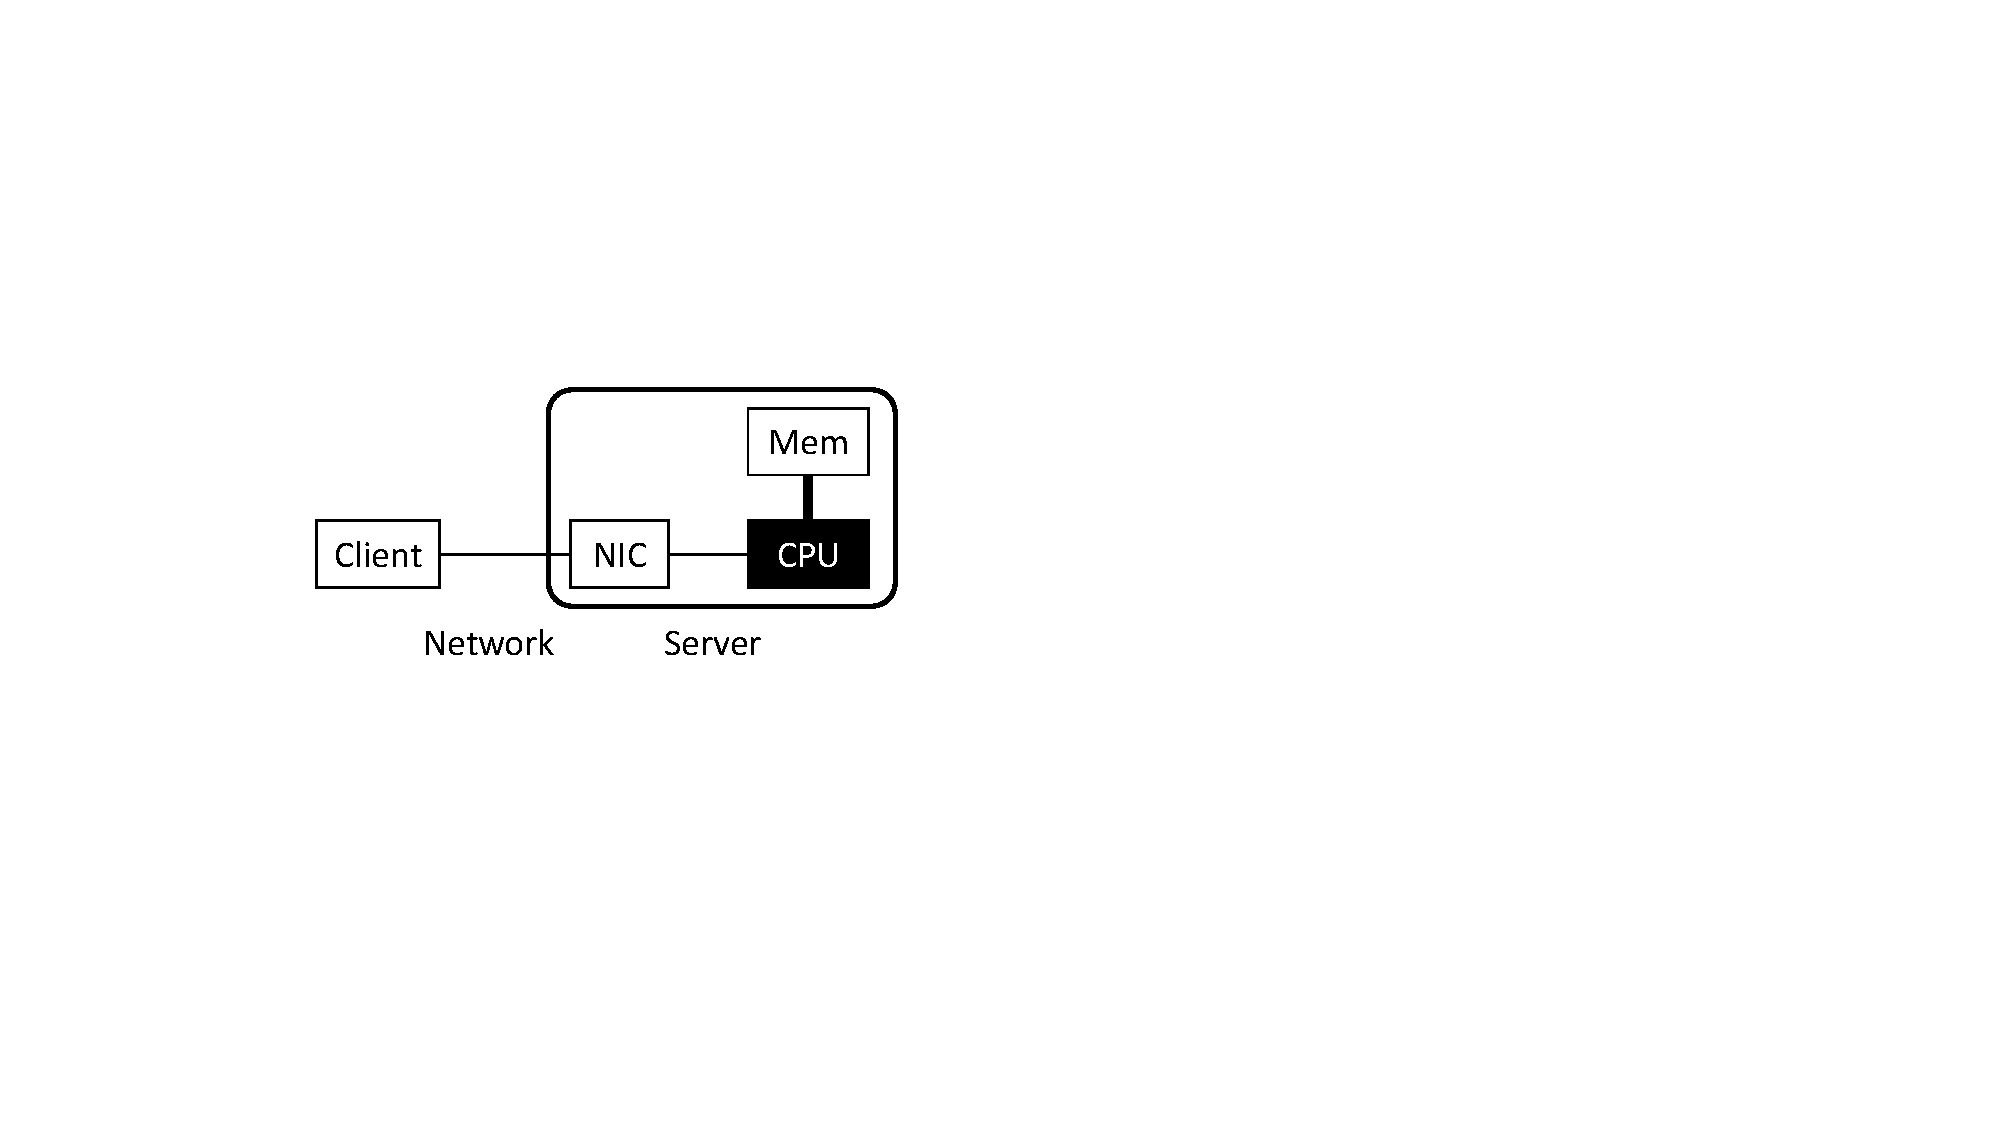
\includegraphics[width=.33\textwidth,page=1]{cropped_access.pdf}}
	\subfloat[One-sided RDMA.\label{kvdirect:fig:memaccess-b}]
	{\includegraphics[width=.33\textwidth,page=2]{cropped_access.pdf}}
	\subfloat[\oursys{}.\label{kvdirect:fig:memaccess-c}]
	{\includegraphics[width=.33\textwidth,page=3]{cropped_access.pdf}}
	\caption{Design space of key-value storage data paths and processing devices. Rows represent data paths. A key-value operation (thin line) may require multiple address-based memory accesses (thick line). The black box indicates where key-value processing occurs.}
	\label{kvdirect:fig:memaccess}
\end{figure*}

When network overhead is reduced to the limit, the throughput bottleneck of high-performance key-value storage systems can be attributed to the latency in key-value operations and random memory access. CPU-based key-value storage requires CPU cycles for key comparison and hash slot calculation. In addition, the key-value storage hash table is several orders of magnitude larger than the CPU cache, so the memory access latency is mainly determined by the cache miss latency under the actual access pattern.

Measurements show that the 64-byte random read latency of modern computers is about 100~ns \footnote{This random read latency assumes a normal page size of 4~KiB, taking into account the latency of TLB misses and data cache line misses.}. The CPU core can issue multiple memory access instructions at the same time, limited by the number of load-store units in the core (such as 3 to 4) \cite {gharachorloo1992hiding,han2010packetshader,zhang2015mega} \footnote{Although there may be dozens of load-store units in each core of the CPU microarchitecture, 64-byte random memory access will cause multiple TLB misses and data cache line misses, so in the actual measurements of this paper, only 3 to 4 random memory access operations can be completed within one memory access latency.}. As shown in Figure \ref{kvdirect:fig:cpu-mem} and Table \ref{kvdirect:tab:kv-cpu-throughput}, in the CPU used in this paper's experiment, each core has a maximum throughput of 29.3~M random 64B accesses per second. On the other hand, the operation of accessing a 64-byte key-value pair usually requires about 100~ns of computation or about 500 instructions, which cannot fit into the instruction window \footnote{The instruction window is the maximum number of instructions that the CPU out-of-order execution engine can rearrange. If there are more than the number of instructions in the instruction window after a memory access instruction, and the memory access latency is greater than the time to execute the number of instructions in the instruction window, then due to the limitation of the instruction window, the pipeline needs to pause (stall) after executing the number of instructions in the instruction window, waiting for the memory access result to return, before it can continue to execute subsequent computation instructions. On the CPU we used, the measured size of the instruction window is about 100 to 200.}. When random memory access and computation are interleaved, due to the instruction window not being able to cover the memory access latency, the performance of the CPU core is reduced to 5.5~M key-value operations (Mops) per second. One optimization method is to aggregate the computation of multiple key-value storage operations before issuing a memory access, and perform memory access in batches \cite {li2016full,narula2014phase}. This optimization can increase the per-core key-value operation throughput of the CPU used in this paper to 7.9~MOps, which is still far lower than the random 64B throughput of the host DRAM.

\begin{figure}[htbp]
	\centering
	\subfloat[Single core.\label{kvdirect:fig:cpu-mem-single}]
	{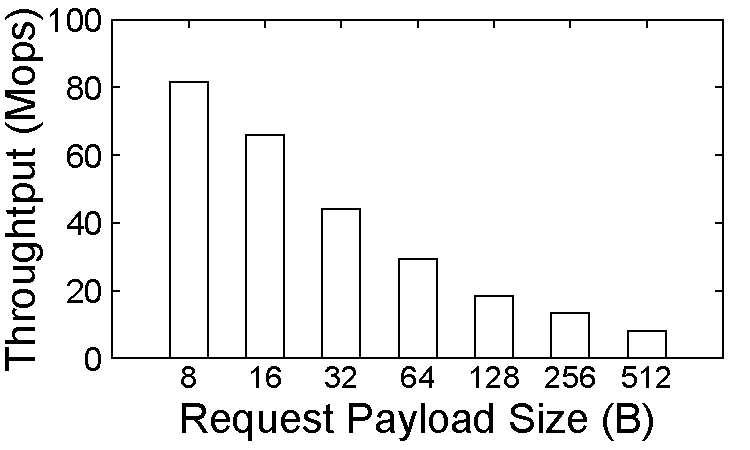
\includegraphics[width=.5\textwidth,page=1]{cpu_random_mem_single_core.pdf}}
	\subfloat[Multi-core.\label{kvdirect:fig:cpu-mem-multi}]
	{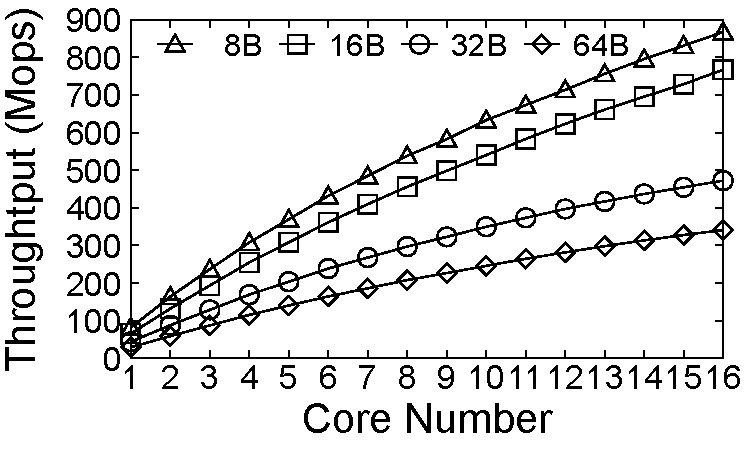
\includegraphics[width=.5\textwidth,page=1]{cpu_random_mem_multi_core.pdf}}
	\caption{CPU random memory access performance.}
	\label{kvdirect:fig:cpu-mem}
\end{figure}


\begin{table}[htbp]
	\small
	\centering
	\caption{Throughput (millions of operations per second) under different workloads and memory access granularities.}
	\begin{tabular}{|c|c|c|c|c|c|c|}
		\hline
		\multirow{2}{*}{Size (bytes)} & \multirow{2}{*}{Computation only} & \multirow{2}{*}{Memory access only} & \multicolumn{4}{c|}{Computation and memory access (batch size)} \\\cline{4-7} 
		&  & & 1 & 2 & 3 & 4 \\\hline
		32 & 24.1 & 44.0 & 7.5 & 11.1 & 13.1 & 14.1 \\\hline
		64 & 11.1 & 29.3 & 5.5 & 6.7 & 7.6 & 7.9 \\\hline
		128 & 5.4 & 18.3 & 3.5 & 4.1 & 4.3 & 4.1 \\\hline
		256 & 2.7 & 13.2 & 2.1 & 2.2 & 2.2 & 2.1 \\\hline
		512 & 1.3 & 8.2 & 1.2 & 1.1 & 1.2 & 1.1 \\\hline
	\end{tabular}
	\label{kvdirect:tab:kv-cpu-throughput}
\end{table}


Observing the limited capacity of the CPU in key-value processing, recent work has used one-sided RDMA to offload key-value processing to the client. One-sided RDMA provides an abstraction of remote access to shared memory. The server-side application registers a block of memory with the local RDMA network card for shared memory. When the client application needs to read and write this shared memory, it sends an RDMA read or write work request to the local RDMA network card. The client RDMA network card converts the work request into a network packet and sends it to the server RDMA network card. The server RDMA network card converts the received packet into a PCIe DMA request, accesses the shared memory, and returns the result to the client RDMA network card. The client RDMA network card sends the read data to the application's memory buffer through PCIe DMA, and then notifies the application through work completion. In this process, the server-side RDMA network card handles read and write requests, completely bypassing the server-side CPU \footnote{In the modern data center server architecture, this statement is not rigorous, because the PCIe root complex and memory controller are both inside the host CPU, and the network card accesses the host memory through PCIe DMA must go through the CPU. This paper's "bypassing the CPU" follows the customary usage in the system academic community, which is a logical meaning, that is, bypassing the software processing on the CPU core. In the system architecture diagram of this paper, the CPU also refers to software processing. The term "bypassing the CPU" will appear many times in the following text, all with this meaning.}.

Although RDMA network cards provide high message throughput (8 to 150~Mops \cite {kalia2016design}), finding an efficient match between RDMA primitives and key-value operations is a challenge. For write (PUT or atomic) operations, multiple network round trips and multiple memory accesses may be required to query the hash index, handle hash conflicts, and allocate variable-sized memory. RDMA does not support transactions. To maintain the consistency of data structures, clients must synchronize with each other, using RDMA atomic operations or distributed atomic broadcasts \cite{szepesi2014designing}. Both of these schemes generate communication overhead and synchronization latency \cite {mitchell2013using,dragojevic2014farm}. Therefore, most RDMA-based key-value stores \cite {mitchell2013using,dragojevic2014farm,kalia2014using} suggest using one-sided RDMA only for GET (read-only) operations. For write (PUT or atomic) operations, they fall back to using the server CPU for processing. Therefore, the throughput of write-intensive workloads is still limited by the bottleneck of the server CPU.

\iffalse
\subsection{FPGA Programmable Network Card}
\label{kvdirect:sec:programmable-nic}

A decade ago, as the speed of processor frequency expansion slowed, people turned to multi-core and concurrency \cite {sutter2005free}. Today, power limits mean that multi-core expansion has also encountered difficulties \cite {esmaeilzadeh2013power}. People are now turning to domain-specific architectures (DSA) for better performance.

%On the spectrum of hardware programmability and performance, general-purpose processors lie on the programmability end, while application-specific integrated circuits (ASICs) lie on the performance end.
%Field-programmable gate array (FPGA) is an architecture between the two extremes, providing both programmability and performance~\cite{bacon2013fpga}.
%As its name indicates, FPGA is a sea of gates.
%Millions of reconfigurable gates and thousands of small block RAMs (BRAMs) provide massive parallelism to build thousands of ``cores'' running simultaneously, and more importantly, customized interconnections among the ``cores'' and BRAMs specializing communication and synchronization for a certain application.
%Consequently, for applications with sufficient bit-level and task-level parallelism, FPGAs provide not only high throughput and power efficiency, but also low and predictable latency.

Due to the increasing mismatch between network speed and CPU network processing capabilities, programmable network cards with FPGA \cite {vfp,greenberg2015sdn,li2016clicknp,caulfield2016cloud} can now be deployed on a large scale in data centers. The core of the programmable network card used in this paper is FPGA, with an embedded network card chip to connect to the network. Programmable network cards usually come with onboard DRAM as a packet buffer and runtime memory for network card firmware \cite {li2016clicknp}, but DRAM is usually not enough to accommodate the entire key-value store.
\fi

\subsection{Challenges Faced by Remote Direct Key-Value Access}
\label{kvdirect:sec:challenge}

KV-Direct moves key-value processing from the CPU to the programmable network card in the server (Figure \ref {kvdirect:fig:memaccess-c}). Like RDMA, the KV-Direct network card accesses host memory via PCIe. PCIe is a packet-switched network with a round-trip latency of about 500 ns and a theoretical bandwidth of 7.87~GB/s per Gen3 x8 endpoint. In terms of latency, because the FPGA hard core used in this paper has an additional processing delay of about 300~ns, the programmable network card reads host memory that has been cached by the CPU via PCIe DMA, with a latency of 800~ns. When randomly DMA reading uncached host memory, there is an additional average delay of 250~ns due to DRAM access, DRAM refresh, and PCIe response reordering in the PCIe DMA engine (Figure \ref {kvdirect:fig:dma-lat}). In terms of throughput, each DMA read or write operation requires a PCIe transport layer packet (TLP) with a 26-byte header and padding for 64-bit addressing. For a PCIe Gen3 x8 network card that accesses host memory at a granularity of 64 bytes, the theoretical throughput is therefore 5.6~GB/s or 87~Mops.

\begin{figure}[t]
	\centering
	\subfloat[DMA throughput.\label{kvdirect:fig:dma-tput}]
	{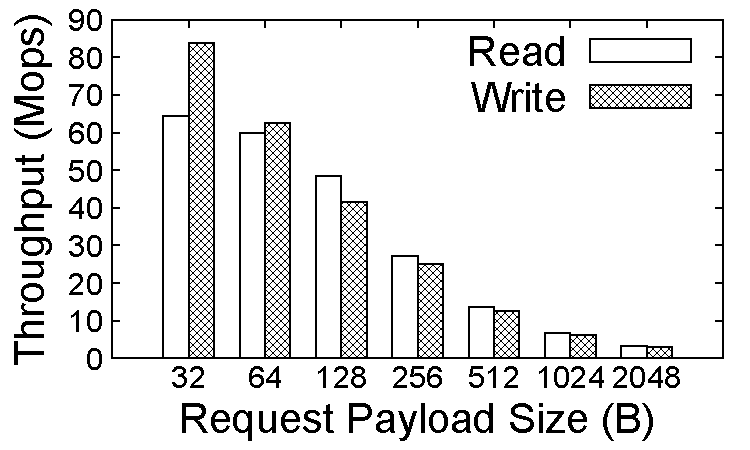
\includegraphics[width=.5\textwidth,page=1]{pcie_bw.pdf}}
	\subfloat[DMA read latency.\label{kvdirect:fig:dma-lat}]
	{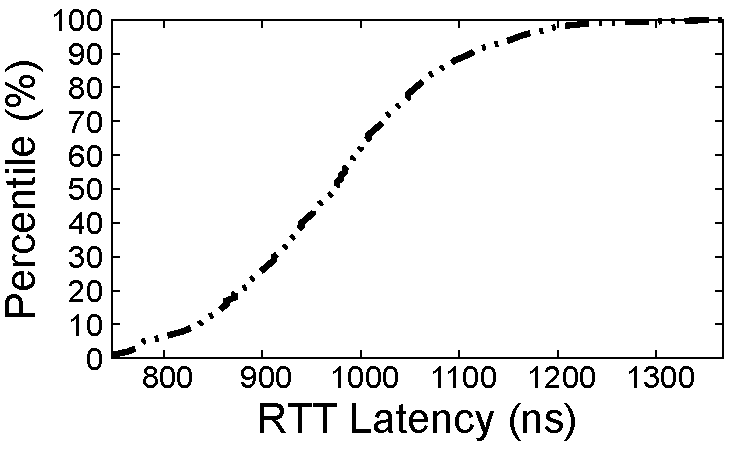
\includegraphics[width=.5\textwidth,page=1]{pcie_latency.pdf}}
	\caption{Random PCIe DMA performance.}
	\label{kvdirect:fig:dma-perf}
\end{figure}

To saturate the throughput of the PCIe Gen3 x8 interface using 64-byte DMA requests, considering a latency of 1050~ns, 92 concurrent DMA requests are needed. However, two practical factors further limit the concurrency of DMA requests. First, the number of requests being processed for each type of DMA is limited by PCIe credit-based flow control. The PCIe root complex in the server announces 88 PCIe transport layer packet (TLP) credits for DMA posted operations and 84 TLP credits for DMA non-posted operations. This means that the number of concurrent write operations cannot exceed 88, and the number of concurrent read operations cannot exceed 84. Second, DMA read operations require the allocation of unique PCIe tags to identify and reorder DMA responses. Although the PCIe protocol and many memory controllers support 256 PCIe tags, the DMA engine in the FPGA used in this paper only supports 64 PCIe tags, further limiting the number of concurrent DMA read requests to 64. This results in a PCIe DMA read throughput of only 60~Mops (million operations per second), as shown in Figure \ref{kvdirect:fig:dma-tput}. On the other hand, for a 40~Gbps network and 64-byte key-value pairs, if the client sends these key-value pairs in batches, the upper limit of network throughput is 78~Mops. This paper aims to saturate network throughput with GET (read) operations. Therefore, the key-value store on the network card must fully utilize the PCIe bandwidth, i.e., the average number of memory accesses per GET operation needs to be close to 1. This boils down to three challenges:

\textbf{Minimize the number of DMA requests per key-value operation.} The hash table and memory allocator are the two main components in the key-value store that require random memory access. Previous work suggests using Cuckoo hash, which keeps the number of memory accesses per GET operation close to 1 even under high load factors. However, Cuckoo hash is optimized for read operations. At load factors above 50%, each PUT operation in Cuckoo hash requires multiple memory accesses on average, with high variance. This not only consumes PCIe throughput but also leads to unstable latency for write-intensive workloads.

In addition to hash table lookups, dynamic memory allocation is needed to store variable-length key-values that cannot be inlined in the hash table. To match PCIe and network throughput under write-intensive small key-value workloads (i.e., to nearly fully utilize both), the number of memory accesses for hash table lookups and memory allocation should be minimized.

\textbf{Hide PCIe latency while maintaining consistency.} Consistency is a term in distributed transactions that refers to the property of logical isolation between concurrently executing transactions. Different hardware modules inside a programmable network card process in parallel, forming a distributed system. Since a key-value operation requires multiple memory read-write accesses, when multiple key-value operations are processed concurrently, each key-value operation can be considered a distributed transaction. This paper implements strict serializability, i.e., the result of concurrently executing multiple key-value operations is the same as if they were executed one after another in the order of network input. Strict serializability is the strongest consistency standard for distributed transactions.

In the FPGA platform of this article, the latency of a PCIe DMA operation is about 1 $\mu$s. When the programmable network card processes key-value requests, if it does nothing else while waiting for the DMA read operation to return, then the throughput of the key-value request will only be about 1 Mops, which is obviously unacceptable.
Therefore, high-performance key-value storage on programmable network cards must concurrently execute key-value operations and DMA requests to hide PCIe latency.
However, key-value operations may have dependencies, and not all key-value operations can be executed concurrently.
For example, a GET operation after a PUT operation on the same key needs to return the updated value.
Again, two adjacent atomic increment operations need to wait for the first one to complete before executing the second one.
This requires tracking the key-value operations being processed, and pausing the pipeline in the event of a data hazard, or better designing an out-of-order executor to solve data dependencies without explicitly pausing the pipeline.


\textbf {Allocate load between network card DRAM and host memory.}
An obvious idea is to use the DRAM on the network card as a cache for host memory, but on the network card, the DRAM throughput (12.8~GB/s) is comparable to the achievable throughput of two PCIe Gen3 x8 interfaces (13.2~GB/s).
This article expects to allocate memory access between DRAM and host memory to take advantage of their two bandwidths.
However, compared with host memory (64~GiB), the on-board DRAM is small (4~GiB), so a mixed cache and load scheduling method is needed.

The following will introduce KV-Direct, a new FPGA-based key-value storage system that meets all the above design goals.
